\subsection{The CLAS12 RICH Detector}

The goal of the RICH reconstruction is to provide a Cherenkov angle estimate for each detected photon and intercepted hadron track, to allow subsequent detailed likelihood particle identification algorithms~\cite{rich-nim}. The CLAS12 tracking system defines the trajectory of the hadron track inside the detector, in particular position and angle within the aerogel radiator and impact point on the \MaPMT plane (if any). In the preliminary phase, the RICH reconstruction identified the cluster of hits produced by the charged particle in the sensor plane. The cross-talk signals are identified by means of an amplitude analysis (based on the time-over-threshold information) in conjunction with geometrical constraints, taking into account that a cross-talk hit should be in the proximity of a genuine hit. Hits neither belonging to a cluster nor flagged as cross-talks are considered Cherenkov photon candidates. 

The photon path inside the RICH is reconstructed in two complementary ways, assuming the middle point of the hadron trajectory inside the radiator as the emission point and the hit pixel coordinates as detection point. The first method uses an analytic formula that takes into account the refraction at the aerogel face and is only valid for directly detected photons. It provides an exact solution. The second method uses a ray tracing algorithm that takes into account also the mirror reflections. It provides a numeric solution based on a iterative procedure. Both methods return the reconstructed Cherenkov angle in conjunction with the corresponding aerogel refractive index, that can slighlty vary with respect the nominal value as a function of the unknown photon energy due to the chromatic effect. 

The relevant RICH components (aerogel, mirrors, \MaPMT plane) are converted into ray-tracing planes or spheres where the photon undergoes refraction, reflection or detection. Each ray-tracing element can be independently aligned. The alignment procedure uses as a benchmark the Cherenkov signal generated by electrons, as identified by CLAS12 sub-detectors other than RICH. For these particles, the expected Cherenkov angle is given by the known particle momentum and mass. The position and orientation of the \MaPMT plane is defined by minimizing the average distance matching the RICH clusters to the extrapolated tracks. All other RICH ray-tracing elements can be aligned with respect to the \MaPMT plane by selecting the sub-sample of photons passing through that component. The alignment is made by minimizing the average distance between the ray-traced detection point (RdP) and the corresponding measured \MaPMT hit over the selected sub-sample of photons.

For each hadron track, the ray-tracing algorithm progresses as described in the following, see Fig.~\ref{Fig:RayShow}. A limited ensemble (of the order of 100) of hypothetical photons, called hereafter trials, is traced assuming an initial particle hypothesis, i.e. electron for a particle identified as electron in CLAS12, pion otherwise. A trial photon is assumed to originate at the emission point at a Cherenkov angle $\theta_T$, corresponding to the given particle hypothesis, and at an azimuthal angle $\phi_T$, uniformly distributed around the charged particle trajectory. For each \MaPMT measured hit, the closest trial, whose RdP stays at a distance smaller than 10 cm from the hit, is taken to be the starting point of the iterative ray-tracing procedure. At each step, two test photons are traced by varying the trial angles by the expected angular resolution in the polar $\theta_T \rightarrow \theta_T + \delta \theta$ and azimuthal $\phi_T \rightarrow \phi_T + \delta \phi$ directions, to quantify the displacement of the corresponding RdP, see Fig.~\ref{Fig:RayAlgo}. The distance between the measured hit $H$ and the trial RdP position $T$ in the sensor plane is measured in terms of the displacement of the test photon $D$ to get an estimate of the next angular step. In particular, the scale factor $f$ of the polar angle step $\Delta \theta = f \delta \theta$ is defined by projecting the distance vector $\vec{HT}$ onto the displacement vector: $f=(\vec{HT}\cdot \vec {DT}) / |\vec{DT}|^2$. The same is done for the azimuthal angle $\phi$.

\begin{figure}[t]
\begin{center}
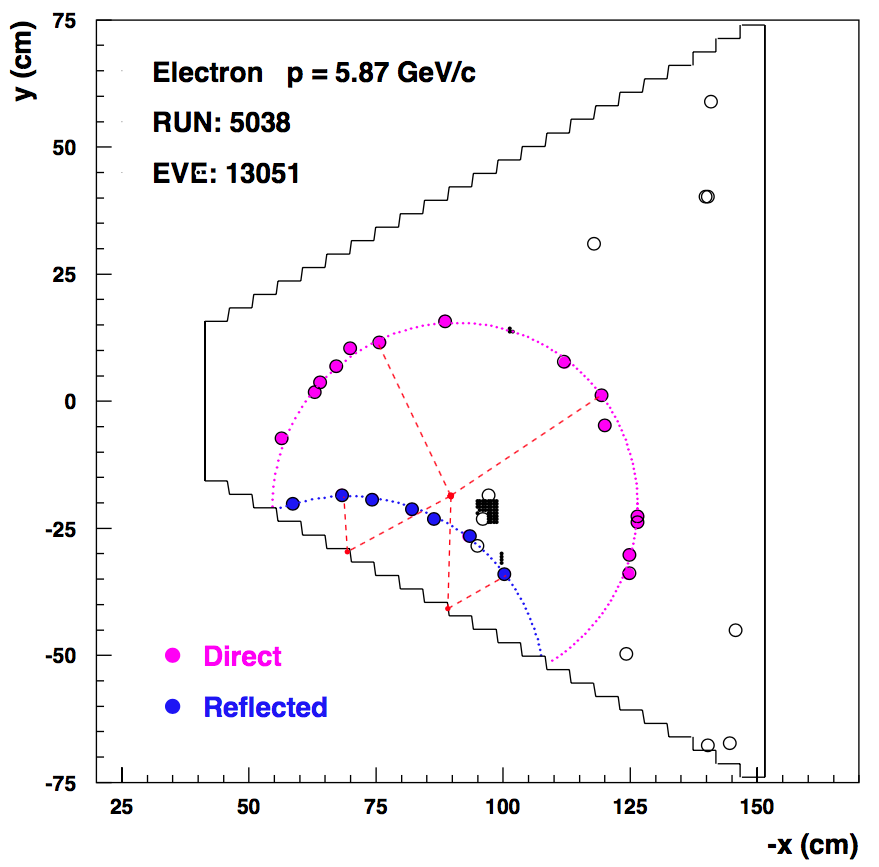
\includegraphics[width=0.8\columnwidth]{pics/example.png}
\end{center}
\caption{Example of ray-tracing. Open circles are the RICH detected hits. The circles are filled in the case that a viable traced solution has been found. Small points indicate the expected pattern for an electron particle, as identified by CLAS12. The dashed lines show examples of the ray-traced photon paths from the common emission point (in the radiator) to the detected hit: two direct photons emitted upwards, two reflected photons emitted downwards. The central cluster is generated by the track impact on the MaPMT plane.}
\label{Fig:RayShow}
\end{figure}

\begin{figure}[t]
\begin{center}
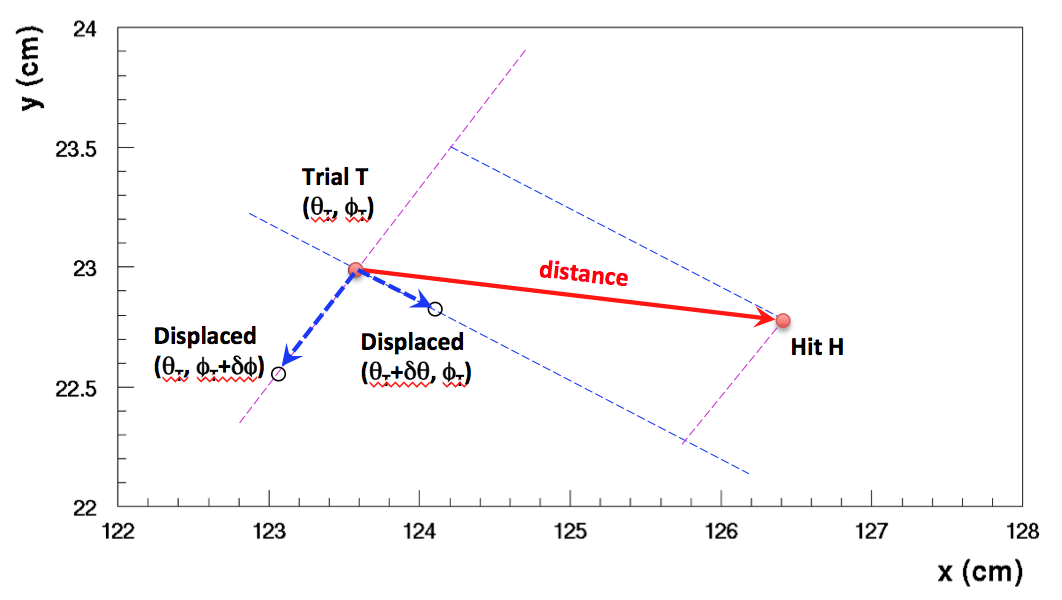
\includegraphics[width=1.0\columnwidth]{pics/ray_trace_example.png}
\end{center}
\caption{Example of the ray-tracing iterative photon path reconstruction. At each step, the emission polar $\theta_T$ and azimuthal $\phi_T$ angles of the trial photon are varied by the expected Cherenkov angle resolution to extrapolate the corresponding displacements of the detection point. The distance between the measured hit and the trial is compared to such displacements to quantify the next angular step.}
\label{Fig:RayAlgo}
\end{figure}


 A new trial photon is traced with the angles changed by such calculated angular shifts ($\theta_T + \Delta \theta$, $\phi_T + \Delta \phi$) and the procedure repeated. At each step the trial RdP gets closer to the measured hit, but an exact solution can not be found as the procedure uses a linear approximation relating the distances in the \MaPMT plane with the angular steps in the 3D space. The iterative procedure stops when the distance of the trial RdP to the measured hit is smaller than a fraction of the \MaPMT pixel size which defines the RICH detector spatial resolution. The converge is fast, typically within 3 steps, so that the average reconstruction time of a RICH event is negligible for CLAS12, at the level of few tens of microseconds.


